\documentclass[a4paper, UTF8]{ctexart}

\usepackage{amsmath}
\usepackage{amssymb}
\usepackage{biblatex}
\usepackage{booktabs}
\usepackage{graphicx}
\usepackage[hidelinks]{hyperref}
\usepackage{listings}
\usepackage{multirow}
\usepackage{warpcol}
\DeclareMathOperator{\sgn}{\mathrm{sgn}}
\lstset{
    basicstyle=\small\tt,
	breaklines=true,
	columns=fixed,
    numbers=left,
	numberstyle=\footnotesize
}
\addbibresource{num2sqrts.bib}

\hypersetup{pdfauthor=zhengxyz123, pdftitle=将某些特定的浮点数转换为特定数学表达式的高效算法}
\title{将某些特定的浮点数转换为形如$\sqrt{a}\pm\sqrt{b}$的数学表达式的高效算法}
\author{zhengxyz123}

\begin{document}
\maketitle

\section{引言}
一些数值计算器在计算分式、根式以及角度时会返回类似$\dfrac{2\sqrt{2}}{3}$或$\dfrac{\pi}{3}$的结果而非浮点数. 它们同样也会显示$1+\sqrt{2}$和$\dfrac{\sqrt{2}+\sqrt{3}}{2}$. 前两者可通过简单的数学运算得出,但是后面两个涉及到了加法运算. 如果我们想分别求出$\sqrt{a}+\sqrt{b}$中的$a$和$b$,最简单的方法是使用二重for循环,但这是效率非常低的方法. 我们是否可以设计一种高效的方法解决上述问题?在本文中,我将介绍一个新的算法将某些特定的浮点数转换为形如$\sqrt{a}\pm\sqrt{b}$的数学表达式. 首先,我将从理论角度分析该算法的可行性;其次,我会将理论转换成实际算法;最后,我会将该算法与其它算法进行比较,并分析各自的优劣.

\section{理论}
我们先讨论没有分母的形式. 为叙述方便,先定义一函数\[S(x,y)=\sgn(x)\sqrt{|x|}+\sgn(y)\sqrt{|y|} \quad\mbox{其中}x,y\in\mathbb{Z}\]在本文中,我们已知浮点数$n$与$S(a,b)$近似相等(即两数之差小到可以忽略),但$a$、$b$未知. 我们的目的是求出特定的$a$和$b$使$|S(a,b)-n|\leq\varepsilon$,其中$\varepsilon$是一个很小的数. 换句话来说,我们希望找到$S(x,y)$的反函数$P(x)$.

当然,使用既定公式求出$P(x)$是不可能的. 唯一可行的途径是穷举搜索. 使用不同的方法进行穷举都可以获得正确的结果,但效率的差异可能是巨大的. 在下文中,我将介绍一种效率较高的方法.

假如我们知道两数之和$p+q$,以及他们的均值$m=\dfrac{p+q}{2}$,那么可以知道$|m-p|=|m-q|$.

同样的,如果已知$n=S(a,b)$, 我们可以从$\dfrac{n}{2}$开始向$\pm\infty$方向分别搜索. 一旦确定了$a$就可以知道唯一的$b$,最后我们仅仅需要一些额外的判断就能得知它们是否为所求.

当然,使用$\dfrac{n}{2}$作为初始值是不合适的,因为我们需要的结果是两个整数. 使用截尾取整后的$\left(\dfrac{n}{2}\right)^2$更适合.

不过,我们可以计算出$\left(\dfrac{\sqrt{100}+\sqrt{101}}{2}\right)^2\approx100.499$,它会舍入到100,这样的设计也是有漏洞的. 但是,有如下极限\[\lim_{x\to+\infty}\left(\frac{\sqrt{x}+\sqrt{x+1}}{2}\right)^2-x=\frac{1}{2}\]它表示函数$f(x)=\left(\dfrac{\sqrt{x}+\sqrt{x+1}}{2}\right)^2$可以近似成$x+\dfrac{1}{2}$.

这样,即使$S(a,b)$中的$a$、$b$的差值很小我们也能分别求出它们.

根据以上的分析,我们可以这样计算初始值
\[
    start(n)=
    \begin{cases}
        \lfloor(\frac{n}{2})^2\rfloor+\frac{1}{2}  &n>0 \\
        -\lfloor(\frac{n}{2})^2\rfloor-\frac{1}{2} &n<0
    \end{cases}
\]

为了书写方便,下面规定一负数的平方根是其绝对值平方根的相反数.

已知$n=S(a,b)$,初始值$\text{start}=start(n)$,令$\text{step}=0.5$并找到第一个数字\[p=\text{start}-\text{step}\]接着就能求出第二个数字\[q=\frac{n}{2}-|\sqrt{p}-\frac{n}{2}|\]$q$必须是一个整数,我们接下来还要做如下操作\[q=\sgn(q)\sqrt{\mathrm{round}(q^2)}\]其中 \verb|round| 表示舍入到最近的整数.

如果$|\sqrt{p}+\sqrt{q}-n|\leq\varepsilon$,其中$\varepsilon$表示一个很小的数,那么$p$和$q$就是所求的$a$和$b$. 否则我们令$\text{step}=\text{step}+1$,继续向正无穷方向搜索.

\section{实现}
以下是本算法的Python实现.

\begin{lstlisting}[language=python, name=example1]
import math

def num2sqrts(n, max_num=1000):
    if n >= 0:
        mid = math.floor((n / 2) ** 2) + 0.5
    else:
        mid = math.ceil(-(n / 2) ** 2) - 0.5
    fsqrt = lambda n: math.copysign(math.sqrt(math.fabs(n)), n)
    actual_mid = n / 2
    t = 0.5
    while True:
        a = fsqrt(mid + t)
        d = math.fabs(a - actual_mid)
        b = actual_mid - d
        b = fsqrt(math.copysign(round(b ** 2), b))
\end{lstlisting}
理论上来说,该算法可以一直执行,直到找到正确的结果. 但是考虑到实际情况,我们必须有一个停止条件.
\begin{lstlisting}[language=python, name=example1]
        if abs(a ** 2) > max_num or abs(b ** 2) > max_num:
            return
        if math.isclose(a + b, n, rel_tol=1e-12):
            return int(round(math.copysign(a ** 2, a))), \
                int(round(math.copysign(b ** 2, b)))
        t += 1
\end{lstlisting}
最后,函数 \verb|num2sqrts| 以长度为2的元组作为结果. 若返回 \verb|None|,这表示程序没有找到正确的结果.

如果没有找到结果,那么可以猜测原浮点数是一个形如$\dfrac{\sqrt{a}+\sqrt{b}}{c}$的分数,我们可以通过穷举分母来解决.

为了展示算法的表现,我令$x\in[-100,100]$和$y\in[-100,100]$,接着记录算法需要多少次循环可求出$S(x,y)$中的$x$和$y$,最后把它们以不同的颜色标识(见图 \ref{fig:perform1}). 可见,当$x$、$y$之差越大时,需要执行更多次的循环.

\begin{figure}[t]
    \centering
    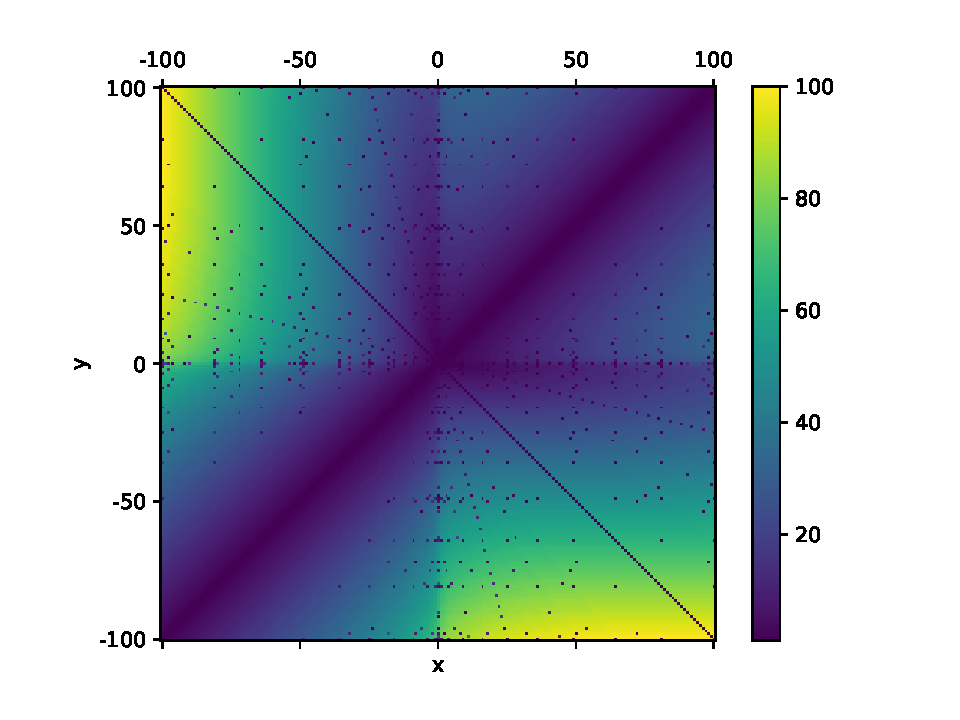
\includegraphics[width=0.8\linewidth]{perform.pdf}
    \caption{算法的表现}
    \label{fig:perform1}
\end{figure}

不过当我们运行如下(或类似)语句时
\begin{lstlisting}[language=python]
num2sqrts(2 * math.sqrt(123))
\end{lstlisting}
函数返回\verb|(492, 0)|,循环执行了438次. 不过$2\sqrt{123}$这个结果可以用一个更简单的算法找到,故我将图 \ref{fig:perform1} 中一、三象限对角线上的值全部赋值为1.

\section{比较}
使用嵌套的for循环(我称其为 \verb|normal_one| 算法)同样也可以求出两根式之和. 让两种算法分别求出$\sqrt{a}+\sqrt{b}$,其中$a$和$b$从0到100的整数中随机选取,并各运行5000遍先记录下运行总时间,再计算出运行一次的平均时间(见表 \ref{tab:comp}). 可见,\verb|num2sqrts| 比纯粹的穷举快了约60倍,而且随着范围的扩大,效率可能会进一步地提高.

\begin{table}[b]
	\centering
	\begin{tabular}{cP{2.6}P{4.4}P{2.1}}
		\toprule
		算法 &
		\multicolumn{1}{c}{总时间/$s$} &
		\multicolumn{1}{c}{平均时间/$\mu s$} &
		\multicolumn{1}{c}{用时之比} \\
		\midrule
		\verb|normal_one| & 18.594490 & 3718.8979 & 60.7 \\
		\verb|num2sqrts|  &  0.306463 &   61.2926 &  1.0 \\
		\bottomrule
	\end{tabular}
	\caption{两种算法效率的比较,在Python 3.11.2下测试}
	\label{tab:comp}
\end{table}

使用PSLQ\cite{ferguson1991}等整数关系探测算法可以找到一个系数是整数的多项式方程,它的根正好等于一个已知浮点数.

例如可以找到$1+\sqrt{2}$是$x^2-2x-1=0$的一根,那么可以通过构造一元二次方程的求根公式来得出$1+\sqrt{2}$.

对于更一般的情况,即两个根式的和或差,它们是四次方程的根. 例如$\sqrt{2}+\sqrt{3}$是$x^4-10x^2+1=0$的一根(虽然它也是$x^2-2\sqrt{2}x-1=0$的一个根,但是这个方程的系数不全是整数,当前的算法并不适用),但构造一元四次方程的求根公式异常麻烦,故这种方法不能适用所有场合.

同时,这些整数关系探测算法也可以将浮点数转换为更复杂的数学表达式,例如mpmath\cite{mpmath}的 \verb|mpmath.identify| 函数:
\begin{lstlisting}[language=python, numbers=none]
>>> import mpmath, sympy
>>> s = mpmath.identify(mpmath.sqrt(2) + mpmath.sqrt(3))
>>> s
'sqrt(((10+sqrt(96))/2))'
>>> sympy.simplify(s)
sqrt(2*sqrt(6) + 5)
\end{lstlisting}
但是,参照上述的运行结果,问题则变成了化简双重根号,就需要编写化简双重根号的程序了,这里就不涉及了.

\section{结论}
在这篇文章中,我介绍了 \verb|num2sqrts| 算法,它可以将一些浮点数转换为与之近似相等的、具有特定形式的数学表达式. 同时,该算法简单、快速,适合应用在科学计算器中.

\printbibliography[title={参考文献}]

\end{document}
